\textbf{信道划分介质访问控制分为以下4种。}

{\textbf{1.频分多路复用}}

将一条信道分割成多条不同频率的信道,就类似于将一条马路分割成多个车道,尽管同一时间车辆都在这条马路上行驶,但是分别行驶在不同的车道上,所以不会发生冲突。现在假设每个车道的宽度不能改变了,但是需要加车道,所以马路就必须变宽,类似于使用频分复用时,如果复用数增加,那么信道的带宽(此时的带宽是频率带宽,不是数据的发送速率)必须得增加。

{注意:每个子信道分配的带宽可以不相同,但它们的总和一定不能超过信道的总带宽(可联想人行道和机动车道是不一样宽的)。在实际应用中,为防止子信道之间的干扰,相邻信道之间要加入``保护频带''(可联想人行道与机动车道、机动车道与机动车道之间的栏杆的作用)。}

\textbf{{2.时分多路复用}}

假设现在只有一个玩具,却有10个小孩要玩,这时候只能将一个固定的时间分割成10份,10个小孩轮流玩这个玩具,即时分多路复用。

所以当使用时分多路复用时,复用数增加并不需要加大信道带宽,只需将每个信道分得的时间缩小即可。也许很多人在这里会有疑问,如果恰好某个时间轮到一个小孩玩了,但是这个小孩现在睡着了,岂不是这段时间就浪费了吗?没错,是浪费了,这时候就需要把时分复用改进,于是引入\textbf{统计时分复用}。继续上面的例子,现在如果该玩具轮到某个小孩玩,但是他睡着了,立刻跳过他,给下一个小孩玩,这样就基本可以保证玩具没有空闲时刻。可见每个孩子下次轮到自己玩的时间都是不确定的,如果睡觉的人多了,很快就轮到了;如果睡觉的人少,就很慢。因此,\textbf{统计时分复用是一种动态的时间分配}(会考选择题,请记住),同时又是异步的(每个孩子玩玩具的时间周期是不固定的),所以统计时分复用又称为异步时分复用。而普通的时分复用就是同步时分复用(因为每个孩子都在一个固定的周期才能得到玩具,即使中间有孩子睡觉也要等)。

\textbf{{3.波分多路复用}}

波分多路复用就是光的频分多路复用,在一根光纤中传输多种不同频率(波长)的光信号,由于各路光的频率(波长)不同,因此各路光信号不互相干扰。最后,再用分波器将各路波长不一样的光分解出来。

\textbf{{4.码分多路复用}}

码分多路复用又称为码分多址(CDMA),它既共享信道的频率,又共享时间,是一种真正的动态复用技术。本书主要讲解CDMA原理中的一个考点,其他内容考研不会涉及,有兴趣的考生可参考教材上的详细讲解。考点分析如下。

\textbf{概念:}每个站点都维持一个属于该站点的芯片序列,并且是固定的。假如站点A的芯片序列为00011011,则A站点发送00011011表示发送比特1;而将00011011每位取反,即发送11100100表示发送比特0。习惯将芯片序列中的0写为-1,1写为+1,所以A站的芯片序列就是(-1
-1 -1 +1 +1 -1 +1
+1),一般将该向量称为该站的码片向量。以下两个定理记住即可。

1)任意两个不同站的码片向量正交,即任意两个站点的码片向量的规格化内积一定为0。\\
2)任意站点的码片向量与该码片向量自身的规格化内积一定为1;任何站点的码片向量和该码片的反码向量的规格化内积一定为-1。

\textbf{考点:某个CDMA站接收到一个碎片序列,怎么去判断是哪站发来的数据,并怎么识别发送了什么信息?见例3-7。}

\textbf{【例3-7】} ~某个CDMA站接收方收到一条如下所示的碎片系列:\\
\hspace*{0.333em} ~ ~ ~ ~ (-1 +1 -3 +1 -1 -3 +1 +1)

假设各个站点的码片向量如下所示。

~ ~ ~ ~ ~ ~站点A:(-1 -1 -1 +1 +1 -1 +1 +1)\\
\hspace*{0.333em} ~ ~ ~ ~ ~站点B:(-1 -1 +1 -1 +1 +1 +1 -1)\\
\hspace*{0.333em} ~ ~ ~ ~ ~站点C:(-1 +1 -1 +1 +1 +1 -1 -1)\\
\hspace*{0.333em} ~ ~ ~ ~ ~站点D:(-1 +1 -1 -1 -1 -1 +1 -1)

{试问:哪些站点发送了数据?分别发送了什么数据?}

解析:此题的解答步骤较为固定,只需将接收到的碎片序列分别与站点A、B、C、D的码片向量进行规格化内积即可。内积为1表示发送了比特1,内积为-1表示发送了比特0,内积为0表示没有发送数据,计算如下。

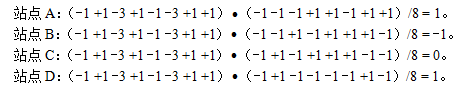
\includegraphics[width=3.70833in,height=0.69792in]{png-jpeg-pics/254FD0619E6D9066C306AD9E400D7922.png}

{由以上计算结果可知,站点A和站点D发送了比特1,站点B发送了比特0,站点C没有发送数据。}
